\documentclass[a4paper,11pt,twocolumn,twoside]{article}
\usepackage{graphicx}
\usepackage{sepln_en}
\usepackage{fullname}
\usepackage[utf8]{inputenc}
\usepackage{booktabs}
\usepackage{tabularx}
\usepackage{todonotes}
% \usepackage[spanish,es-nosectiondot, es-tabla, es-noindentfirst, es-nolists]{babel}

\input epsf

\setlength\titlebox{4in} %esto por defecto

\title{Overview of the eHealth Knowledge Discovery Challenge at IberLEF 2021}

\author {
  \textbf{Alejandro Piad-Morffis,$^{1,*}$},
  \textbf{Suilan Estevez-Velarde$^1$},
  \textbf{Yoan Gutierrez$^{2,3}$}\\
  \textbf{Yudivian Almeida-Cruz$^1$},
  \textbf{Andrés Montoyo$^{2,3}$},
  \textbf{Rafael Muñoz$^{2,3}$}\\
$^1$School of Math and Computer Science, University of Havana, Cuba\\
\texttt{\{apiad,sestevez,yudy\}@matcom.uh.cu}\\
$^2$University Institute for Computer Research, IIUI, University of Alicante, Spain\\
$^2$Department of Language and Computing Systems, University of Alicante, Spain\\
\texttt{\{ygutierrez,montoyo,rafael\}@dlsi.ua.es}\\
}

\seplntranstitle{Resumen de la Tarea de Descubrimiento de Conocimiento en Salud en IberLEF 2021}

\seplnclave{Palabras, palabras, palabras en castellano...}

\seplnresumen{Resumen del artículo en castellano con una sangría a izquierda y
derecha de 1 cm, justificado por ambos lados, con tamaño de fuente
11.}


\seplnkey{Palabras, palabras, palabras en inglés...}

\seplnabstract{Resumen del artículo en inglés con una sangría a izquierda y
derecha de 1 cm, justificado por ambos lados, con tamaño de fuente
11.}

\firstpageno{1}

\begin{document}

% la siguiente instrucción sólo se debe usar si el abstract sobrescribe el texto
% la longitud variará según se necesite

%\setlength\titlebox{20cm} % se aumenta el tamaño del espacio reservado para datos de título

\label{firstpage} \maketitle

%\begin{abstract}
%Resumen del artículo con una sangría a izquierda y derecha de 0.32
%cm, justificado por ambos lados, con tamaño de fuente 11.
%
%\end{abstract}

\section{Introduction}


The accelerated growth of the Internet and the increased production of textual resources in all areas of human endeavour has created both new opportunities and new challenges for the research community.
On one hand, larger datasets can be collected and used to build increasingly powerful machine learning models~(e.g., GPT-3 and related).
On the other hand, is becoming increasingly difficult to organise, categorise, cross-reference, and fact-check the textual information available online.
The ease of access to both publication and consumption of textual information is arguably one of the root causes of the increasingly worrying phenomenon of fake news.

Staying up-to-date on information about topics of interest is crucial in technical or scientific domains.
For this purpose, specialists rely on a combination of curated sources (e.g., domain-specific repositories like arxiv, bioarxiv, semantic scholar) and technologies for search and recommendation (e.g., google scholar).
These resources significantly improve the experience of collecting and consuming large amounts of relevant information on a specific topic.
Tools like Connected Papers~\cite{} and Papers with Code~\cite{} are one step beyond the indexing of documents, providing summarised and structured representations of the content in a collection of documents.
However, it remains an open problem to automatically combine, summarise, and present the relevant information in a collection of documents in a semantic structure~(e.g., a knowledge graph) that allows a specialist to quickly grasp the essential concepts of a specific knowledge field.

A potential solution to this problem would require methods to automatically detect in natural language the most relevant concepts and the factual statements in which they are related, possibly normalise them into well-established taxonomies and classifications, and store them in computational data structures where they can linked with related concepts, e.g., knowledge graphs.
The first step of this process, i.e., the detection of relevant concepts and semantic relations in text, is already a challenging computational task, given the complexity and variability of natural language.
To encourage research and development in this area, several academic competitions have been organised through the years by organisations such as CLEF, SEMEVAL, and more recently, IBERLEF.

In this context, the eHealth Knowledge Discovery Challenge is designed to foster the development of automatic knowledge discovery systems for natural language sentences in a cross-domain and multi-lingual setting.
Concretely, a token-level annotation model of 4 entities and 13 semantic relations is defined, and a corpus of more than 1500 sentences from different factual sources~(i.e., Spanish Medline articles, Spanish Wikinews articles, and English biomedical preprints related to COVID-19) is annotated.
Two computational tasks are defined: the detection of multi-span, non-contiguous, and potentially overlapping named entities; and the detection of semantic relations between them.
A shared annotation campaign was organised, where a total of 9 participants presented 10 different systems with varied levels of performance.

The eHealth-KD task focuses on cross-domain, multi-lingual and low-resource solutions. This setting presents a significant challenge to existing state-of-the-art methods, which often rely on large amounts of training data.
A successful approach to the eHealth-KD must leverage transfer learning across different domains and languages, since the vast majority of the training examples are provided in Spanish language and from the Medline domain, while only a small development set is available in the remaining settings.
With this added complexity, we expect to encourage solutions that can be deployed in low-resource environments, where is unfeasible to train large language models over longs periods of time.

The remaining of this paper is organized as follows.
Section~\ref{sec:task} describes the eHealth-KD tasks in greater detail, including the annotation model and performance metrics.
Section~\ref{sec:resources} describes the corpora and other resources created for this challenge and presents some qualitative analysis of their characteristics.
Section~\ref{sec:systems} describes the different systems presented in the challenge and summarises the main approaches and most common characteristics they share.
Section~\ref{sec:results} presents the main results of the challenge.
Section~\ref{sec:discussion} discusses the most interesting insights of the challenge and highlights both the most relevant lessons learned and potential improvements for future similar endeavours.

\section{Tasks Descriptions}\label{sec:task}

\begin{figure*}[htb]
  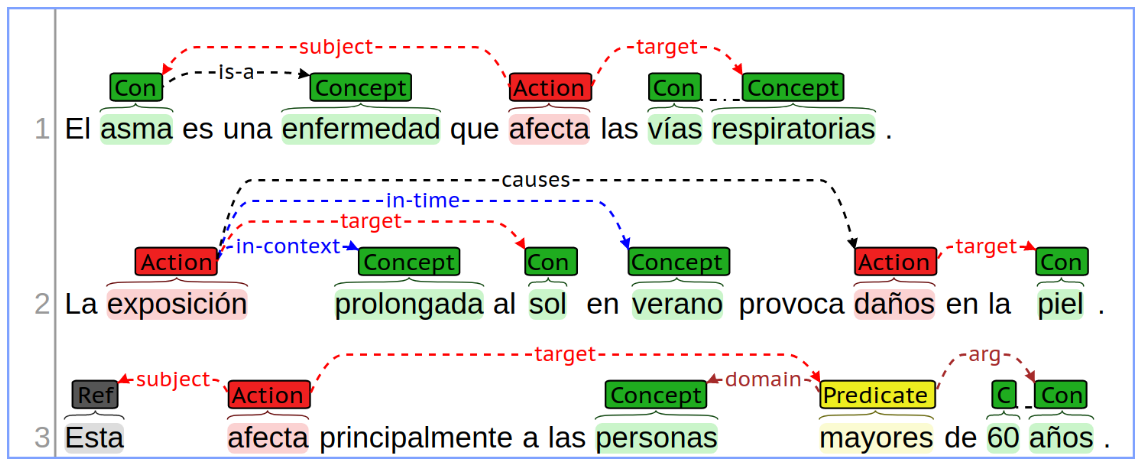
\includegraphics[width=\textwidth]{model.png}
  \caption{Examples the annotation model defined for the eHealth-KD Challenge.\label{fig:model}}
\end{figure*}

The eHealth-KD challenge consists on the automatic sentence-level annotation
of multi-token entities and binary relations among them.
A custom annotation model has been defined, comprising 4 entity types and 13 relations,
that attempts to capture a large part of factual semantics in technical documents,
including encyclopedias, news, and scientific papers. The annotation model is explained in detail in \namecite{piad2019general}. Figure~\ref{fig:model} shows an illustrative example of the annotation model in three Spanish sentences.
The challenge has been divided into two different subtasks: entity recognition and relation extraction.

\subsection{Subtask A: Entity recognition}

The goal of this subtask is to identify all the entities per document and their types. These entities are all the relevant terms (single word or multiple words) that represent semantically important elements in a sentence. Entities always consist of one or more complete words (i.e., not a prefix or a suffix of a word), and never include any surrounding punctuation symbols, parenthesis, etc. There are four types for entities:

\begin{description}
  \item[Concept:] identifies a rel willevant term, concept, idea, in the knowledge domain of the sentence.
  \item[Action:] identifies a process or modification of other entities. It can be indicated by a verb or verbal construction, such as “afecta” (affects), but also by nouns, such as “exposición” (exposition) and “daños” (damages).
  \item[Predicate:] identifies a function or filter of another set of elements, which has a semantic label in the text, such as “mayores” (older), and is applied to an entity, such as “personas” (people) withsome additional arguments such as “60 años” (60 years).
  \item[Reference:] identifies a textual element that refers to an entity --of the same sentence or of different one--, which can be indicated by textual clues such as “esta”, “aquel”, etc.
\end{description}

\subsection{Subtask B: Relation extraction}

Subtask B continues from the output of Subtask A, by linking the entities detected and labelled in the input document. The purpose of this subtask is to recognise all relevant semantic relationships between the entities recognised. The semantic relations are divided in different categories:

\paragraph{General relations (6)} are general-purpose relations between two entities that have a pre-defined semantic:

\begin{description}
  \item[is-a:] indicates that one entity is a subtype, instance, or member of the class identified by the other.
  \item[same-as:] indicates that two entities are semantically the same.
  \item[has-property:] indicates that one entity has a given property or characteristic.
  \item[part-of:] indicates that an entity is a constituent part of another.
  \item[causes:] indicates that one entity provokes the existence or occurrence of another.
  \item[entails:] indicates that the existence of one entity implies the existence or occurrence of another.
\end{description}

\paragraph{Contextual relations (3)} allow to refine an entity by attaching modifiers:

\begin{description}
  \item[in-time:] to indicate that something exists, occurs or is confined to a time-frame.
  \item[in-place:] to indicate that something exists, occurs or is confined to a place or location.
  \item[in-context:] to indicate a general context in which something happens, like a mode, manner, or state.
\end{description}

\paragraph{Action roles (2)} indicate which role play the entities related to an Action:

\begin{description}
  \item[subject:] indicates who performs the action.
  \item[target:] indicates who receives the effect of the action.
\end{description}

\paragraph{Predicate roles (2)} indicate which role play the entities related to a Predicate:

\begin{description}
  \item[domain:] indicates the main entity on which the predicate applies.
  \item[arg:] indicates an additional entity that specifies a value for the predicate to make sense.
\end{description}

\subsection{Evaluation}

To evaluate each subtask, we score correct, incorrect, partial, missing, and spurious
annotations, and weight them according to an $F_1$ measure, independently per task.
Partial annotations~(i.e., where predicted entities overlap with the gold standard) are scored as half the value of correct annotations.

$$Rec = \frac{C_A + C_B + \frac{1}{2} P_A}{C_A + I_A + C_B + P_A + M_A + M_B}$$

$$Prec = \frac{C_A + C_B + \frac{1}{2} P_A}{C_A + I_A + C_B + P_A + S_A + S_B}$$

$$F_1 = 2 \cdot \frac{Prec \cdot Rec}{Prec + Rec}$$

Furthermore, the challenge is graded in three different scenarios:
one scenario for each subtask independently, and a main scenario where both subtasks are performed in sequence, which ultimately decides the winner of the challenge.
In the subtask-specific scenarios, the previous formulas are redefined based only on the relevant subset of annotations for each subtask.

\section{Corpora and Resources}\label{sec:resources}

The Challenge is based on a corpus of documents composed of
sentences taken from previous challenges and other resources,
and newly annotated sentences.
The corpus is divided into three collections: training, development, and testing.
All collections contain sentences extracted from MedlinePlus, Wikinews, and the CORD-19 corpus, related with health topics, but showing a significant variety in terms of format and structure.
Furthermore, the majority of sentences are in Spanish, but a small set of English sentences is also included, to evaluate generalisation across domains.

In the training collection, each sentence is labelled with its corresponding domain and language (Spanish or English), so that participants can potentially fine-tune different models for each domain/language and learn to identify them in the text.
In the development collection, sentences are from all different sources and no labelling is provided, so that participants can evaluate their systems in a similar environment to the testing set.
In the testing set, a large number of unlabelled sentences is added along with a small batch of labelled sentences. This serves to discourage participants from manually labelling the test set.

As in previous edition, the corpus for eHealth-KD 2021 is based mostly on text extracted from \textit{Medline} sources, plus additional resources.
First, the same corpus used in the 2020 edition will be provided for training and development, while a new set of previously unlabelled sentences will be manually annotated and used for the test collection. Additionally, health-related news sourced from \textit{Wikinews} will be also provided for training and development.
Finally, a small set of sentences from scientific papers in the \textit{CORD-19} corpus (in English language) are selected, annotated, and distributed in the development, and testing collections. Overall, the composition of the corpus is presented in Table~\ref{tab:corpus}.

\begin{table}
  \begin{tabular}{lllr}
    \toprule
    \textbf{Collection} & \textbf{Source} & \textbf{Language} & \textbf{Size} \\
    \midrule
    Training & Medline & Spanish & 1200 \\
             & Wikinews & Spanish & 300 \\
    \midrule
    Develop & Medline & Spanish & 25 \\
            & Wikinews & Spanish & 25 \\
            & CORD & English & 50 \\
    \midrule
    Testing & Medline & Spanish & 75 \\
            & Wikinews & Spanish & 75 \\
            & CORD & English & 150 \\
    \midrule
    Total   &      &         & 1900 \\
    \bottomrule
  \end{tabular}
  \caption{Composition of the corpus, highlighting resources from previous
  challenges and newly annotated sentences.\label{tab:corpus}}
\end{table}

\begin{table*}[t!]
  \centering
  \begin{tabularx}{\textwidth}{lXllll}
    \toprule
    \textbf{System} & \textbf{Features} & \textbf{Tasks} & \textbf{Task A} & \textbf{Task B} & \textbf{Multi-span} \\
    \midrule
    Codestrange & Spacy & Only A & Sequence & - & Custom \\
    GuanZhengyi & BETO & Only A & Sequence & - & BIO \\
    IXA & ROBERTa & Sequential & Sequence & Sequence & BIO \\
    JAD & BERT & Joint & Token & Pairwise & Relation \\
    Maoqin & BERT & Only A & Sequence & - & BIO \\
    PUCRJ-PUCPR-UFMG & BERT & Joint & Sequence & Pairwise & BIO \\
    uhKD4 & Word2vec POS-tag Character Position & Sequential & Sequence & Pairwise & BILOUV \\
    UH-MMM & BERT FastText POS-tag Dependency Character & Sequential & Sequence & Pairwise & BILOUV \\
    Vicomtech Joint & BERT & Joint & Sequence & Pairwise & BIO \\
    Vicomtech Seq2Seq & T5 & Joint & Text2text & Text2text & Text \\
    \bottomrule
  \end{tabularx}
  \caption{Summary of the approaches presented at the eHealth-KD Challenge.\label{tab:participants}}
\end{table*}

\section{Systems Descriptions}\label{sec:systems}

The challenge caught the attention of 8 participants from across the globe,
who presented a variety of approaches clustered around deep learning architectures.
Table~\ref{tab:participants} summarises the main characteristics of each approach presented.
A brief summary of each system follows:

  \paragraph{Codestrange} proposes a stadnard NER pipeline trained with the \texttt{spacy} library, modified to fit the eHealth-KD annotation model. They apply some preprocessing steps to deal with multi-token annotations, which are not natively handled by the tool.

  \paragraph{GuanZhengy} presents a traditional NER architecture for Subtask A, based on contextual embeddings from a BETO pre-trained language model, and a combination of Convolutional, Bi-LSTM, and CRF layers for decoding BIO tags~\cite{GuanZhengyi2021}.

  \paragraph{IXA} models both substasks are sequence labelling problems encoded with a BIO system and using a pre-trained XLM-RoBERTa language model. Subtask A is solved with a standard NER architecture. For Subtask B, they solve a sequence labelling problem for each pair of entities, where tags correspond to relation labels~\cite{edgarandres2021}.

  \paragraph{JAD} proposes a single model based on BERT pre-trained embeddings that jointly outputs entity labels~(at token level) and pairwise relation labels. To deal with multi-span entities, they add a virtual relation that links tokens from the same entity~\cite{JAD2021}.

  \paragraph{Maoquin} presents a traditional NER architecture based on BERT pre-trained embeddings and BIO tags for Subtask A, combined with Bi-LSTM and CRF layers~\cite{Maoqin2021}.

  \paragraph{PUCRJ-PUCPR-UFMG} proposes a joint model that outputs token labels~(modelled as a sequence labelling problem) and pairwise relation labels, based on BERT pre-trained embeddings as the main feature~\cite{lucas2021}.

  \paragraph{uhKD4} models both subtasks sequentially, using a standard NER architecture with BILOUV encoding for Subtask A and a pairwise classification model for Subtask B. As features, they employ a variety of syntactic characteristics~(POS-tags, character embeddings, positional embeddings) as well as word2vec embeddings~\cite{uhKD42021}.

  \paragraph{UH-MMM} also models both subtasks sequentially, using a standard NER architecture with BILOUV encoding for Subtask A and a pairwise classification model for Subtask B. As a key characteristic, they encode the shortest dependency path between two entities for the relation prediction. They also compare several different embeddings, including health-specific and general-purpose approaches~\cite{uhmmm2021}.

  \paragraph{Vicomtech} presents two different models. The first consists of a joint architecture for sequence labelling~(Subtask A) and pairwise relation prediction~(Subtask B) based on BERT pre-trained embeddings. The second model is a text-to-text architecture, based on a T5 model, fine-tuned on a problem-specific encoding of the entities and relations that solves both subtasks in a single pass~\cite{vicomtech2021}.

As it can be seen in Table~\ref{tab:participants}, the predominant solution for feature extraction is using pre-trained language models such as BERT and its variants, although some approaches also include classic NLP features.
In contrast with previous editions, the joint approach~(solving both subtasks simultaneously with a shared architecture) is used by more than half of the systems that tackle both subtasks.
As in previous editions, subtask A is commonly modelled as a sequence labelling problem using some variant of the BIO encoding.
Likewise, subtask B is commonly modelled as a pairwise classification problem, by combining all pairs of entities detected in each sentence.

Two approaches stand out as distinctly novel in this edition of the challenge, presented by IXA and Vicomtech, respectively.
The former models subtask B also as a sequence labelling problem, reusing the same architecture as in subtask A.
The latter presents a text-to-text architecture which translates a raw sentence into a semi-structured representation that encodes all the entities and their relations.

\section{Results and Discussion}\label{sec:results}

\begin{table*}
  \resizebox{\textwidth}{!}{
  \begin{tabular}{l|ccc|ccc|ccc}
    \toprule
    & \multicolumn{3}{c|}{\textbf{Main}} & \multicolumn{3}{c|}{\textbf{Task A}} & \multicolumn{3}{c}{\textbf{Task B}} \\
    \textbf{Team}    & $F_1$ & $P$   & $R$   & $F_1$ & $P$   & $R$   & $F_1$ & $P$   & $R$ \\
    \midrule
    Vicomtech        & \bf 0.531 & 0.540 & 0.534 & 0.684 & 0.699 & \bf 0.747 & 0.371 & \bf 0.541 & 0.283 \\
    PUCRJ-PUCPR-UFMG & 0.528 & \bf 0.568 & 0.502 & \bf 0.706 & \bf 0.714 & 0.697 & 0.263 & 0.366 & 0.205 \\
    IXA              & 0.498 & 0.464 & \bf 0.538 & 0.653 & 0.613 & 0.698 & \bf 0.430 & 0.453 & \bf 0.409 \\
    uhKD4            & 0.422 & 0.485 & 0.374 & 0.527 & 0.517 & 0.537 & 0.317 & 0.556 & 0.222 \\
    UH-MMM           & 0.338 & 0.291 & 0.403 & 0.607 & 0.546 & 0.685 & 0.053 & 0.077 & 0.041 \\
    Codestrange      & 0.232 & 0.337 & 0.176 & 0.080 & 0.415 & 0.044 & 0.032 & 0.437 & 0.017 \\
    JAD              & 0.109 & 0.234 & 0.071 & 0.262 & 0.315 & 0.224 & 0.007 & 0.375 & 0.003 \\
    GuanZhengyi      & -     & -     & -     & 0.334 & 0.520 & 0.245 & -     & -     & -     \\
    Maoqin           & -     & -     & -     & 0.173 & 0.271 & 0.127 & -     & -     & -     \\
    \midrule
    \it human        & 0.644 & 0.673 & 0.618 & 0.831 & 0.862 & 0.802 & 0.621 & 0.596 & 0.647 \\
    \it baseline     & 0.232 & 0.337 & 0.176 & 0.306 & 0.350 & 0.271 & 0.032 & 0.437 & 0.017 \\
    \bottomrule
  \end{tabular}}
    \caption{Summary of results in the three evaluation scenarios of the eHealth-KD Challenge. The top result in every metric is highlighted. For comparative purpose, an estimated \textit{human} performance~(based on inter-annotator agreement) and a simple computational \textit{baseline} are also reported.\label{tab:results}}
  \end{table*}

Table~\ref{tab:results} summarises the main results obtained by all participants in the eHealth-KD 2021 Challenge.
In the main scenario the best performing system was the joint architecture presented by Vicomtech, followed closely by a very similar architecture presented by PUCRJ-PUCPR-UFMG.
Both approaches are based on the previous edition's winner, further confirming the hypothesis that using end-to-end architectures for solving both subtasks simultaneously outperforms task-specific architectures.
This advantage seems to be mostly due to the strength of these solutions for solving subtask A, since in subtask B the best performing system is the sequence labelling architecture presented by IXA.

As expected by the relative complexity of the tasks, results for subtask A are significantly better than for subtask B.
However, neither subtask can be said to be fundamentally solved up to human performance.
The human benchmark, estimated by inter-annotator agreement, is approximately $11.3$,
$12.5$, and $19.1$ percent points above the best performing systems in each scenario, respectively.
This indicates that there is still a significant margin for improvement, especially on the relation extraction subtask.

The use of pre-trained language models seems to provide a significant advantage, taking into consideration the complexities of dealing with multiple domains and languages.
By leveraging multi-lingual models, most systems are capable of dealing with English sentences even though there is little to no training data~(i.e., only 50 English sentences were provided in the development collection).
However, there is a gap in performance across domains and languages, as shown by Table~\ref{tab:models}.
Most participants have a better performance on the subset of the test collection that corresponds to the \textit{Medline} and \textit{Wikinews} sources, and a correspondingly worse performance on the \textit{CORD} subset.
On average, performance on \textit{Medline}~(the most common source) is $25.2$ and $15.2$ percent points higher than on \textit{CORD}~(the least common source) for subtask A and B, respectively.
This suggests that multilingual pre-trained models alone are insufficient as an effective transfer learning method in low-resource scenarios such as the one presented in this challenge.

\begin{table*}
  \resizebox{\textwidth}{!}{
  \begin{tabular}{l|rrrr|rrrr|rrrr}
    \toprule
    & \multicolumn{4}{c|}{\textit{Medline}} & \multicolumn{4}{c|}{\textit{Wikinews}} & \multicolumn{4}{c}{\textit{CORD}} \\
    & \multicolumn{2}{c}{\textbf{Task A}} & \multicolumn{2}{c|}{\textbf{Task B}} & \multicolumn{2}{c}{\textbf{Task A}} & \multicolumn{2}{c|}{\textbf{Task B}} & \multicolumn{2}{c}{\textbf{Task A}} & \multicolumn{2}{c}{\textbf{Task B}} \\
    \textbf{Team} & $F_1$ & \textit{Diff} & $F_1$ & \textit{Diff} & $F_1$ & \textit{Diff} & $F_1$ & \textit{Diff} & $F_1$ & \textit{Diff} & $F_1$ & \textit{Diff} \\
    \midrule
Vicomtech        & 0.843 &  0.156 & 0.467 & 0.093 & 0.794 & 0.106 & 0.478 &  0.104 & 0.576 & -0.111 & 0.256 & -0.118 \\
PUCRJ-PUCPR-UFMG & 0.779 &  0.071 & 0.374 & 0.109 & 0.781 & 0.073 & 0.362 &  0.098 & 0.641 & -0.067 & 0.170 & -0.095 \\
IXA              & 0.699 &  0.045 & 0.562 & 0.130 & 0.714 & 0.060 & 0.493 &  0.062 & 0.609 & -0.045 & 0.338 & -0.094 \\
uhKD4            & 0.772 &  0.242 & 0.538 & 0.219 & 0.714 & 0.184 & 0.431 &  0.112 & 0.348 & -0.182 & 0.127 & -0.192 \\
UH-MMM           & 0.692 &  0.081 & 0.158 & 0.104 & 0.695 & 0.083 & 0.061 &  0.006 & 0.538 & -0.073 & 0.014 & -0.041 \\
Codestrange      & 0.177 &  0.096 & 0.138 & 0.105 & 0.124 & 0.042 & 0.008 & -0.025 & 0.017 & -0.065 & 0.000 & -0.033 \\
JAD              & 0.238 & -0.025 & 0.036 & 0.028 & 0.243 & -0.02 & 0.000 & -0.007 & 0.280 &  0.017 & 0.000 & -0.007 \\
GuanZhengyi      & 0.807 &  0.470 & 0.000 & 0.000 & 0.286 & -0.05 & 0.000 &  0.000 & 0.000 & -0.336 & 0.000 &  0.000 \\
Maoqin           & 0.266 &  0.094 & 0.000 & 0.000 & 0.269 & 0.097 & 0.000 &  0.000 & 0.000 & -0.172 & 0.000 &  0.000 \\
    \midrule
    Mean difference &       &  0.136 &       & 0.087 &       & 0.063 &       &  0.038 &       & -0.114 &       & -0.064 \\
    \bottomrule
  \end{tabular}}
  \caption{Individual results per domain in subtasks A and B. The \textit{Diff} column corresponds to the absolute difference between the presented $F_1$ and the aggregated $F_1$ on the corresponding scenario,
  as reported in Table~\ref{tab:results}. A positive \textit{Diff} indicates that team had a correspondingly better result on that specific subset than in the overall corpus.\label{tab:models}}
\end{table*}

Modelling both subtasks independently seems to be less effective than using some form of shared architecture.
The three best performing systems exploit in some manner the interrelation between both subtasks, either by using a single architecture with separate outputs~(thus sharing a large part of the feature extraction model), or by reusing the same architecture in both subtasks.
In contrast, systems that attempt to solve subtask B based on structured information obtained from subtask A have a significant drop in performance in this task.
This suggests that subtask B also benefits from direct access to the raw sentence, which cannot be effectively captured with position embeddings or dependency subtrees alone.

One surprising result is that the best performing system in subtask B uses a sequence labelling approach, as opposed to the most commonly deployed pairwise classification model.
IXA's approach for subtask B consists in feeding a regular NER architecture~(the same one used for subtask A) with a raw sentence, where two entities of interest are marked.
The model is trained to output a BIO sequence where tags are aligned with the marked entities and correspond to the label of the relation among them, if any.
This requires $O(|E|^2)$ queries to the model for each sentence with $|E|$ entities detected.
We believe this approach can be improved by training the model with all entities at once, predicting one-to-many relations in a single pass, thus reducing the complexity to $O(|E|)$ per sentence.

A second promising approach for subtask B is presented by Vicomtech, although it didn't obtain competitive enough results.
This approach consists of a text-to-text architecture, fine-tuned from a T5 language model on the task of translating from raw sentences to a semi-structured output that encodes the result of both subtasks.
The output structure consists of a list of tuples with all the pairs of entities detected and their corresponding relations.
However, being a text-to-text model, it suffers from hallucination, which requires some post-processing to fix.
Furthermore, the output structure still contains unnecessary redundancy~(the same entities need to be predicted for every relation in which they appear).
However, we believe that this is a fruitful direction for future research that should be explored in greater depth.

Moving towards a full solution to the eHealth-KD challenge, there are some fundamental obstacles that still need to be tackled.
The most salient one is effectively capturing the interaction between entities and the semantic relations in which they appear.
As we have learned from observing human annotators, they usually annotate simultaneously entities and relations.
Furthermore, they do not follow the left-to-right natural order of the sentence, but rather annotate the most salient entities first~(e.g., the main Action and related Concepts) and then add the contextual relations and supporting entities.
Althought it is unclear whether this strategy is necessary, it presents an interesting alternative approach for designing an automatic annotation system in the form of an agent that performs annotation actions on the sentence, perhaps trained with a reinforcement learning approach.
For this purpose, it could be interesting to analize not only the final annotated sentence but the individual annotation events that human annotators produce, including the undoing previous annotations.

The four editions of the eHealth-KD challenge have shown that knowledge discovery in natural language text is still an open and challenging problem.
Detecting the most relevant entities and relations is but a first step in a hypothetical knowledge discovery system that could be used to intelligently explore the vast amount of information available in natural language.
Moving up in this pipeline, the next natural step is to create semantic structures~(e.g., knowledge graphs) that integrate the entities and relations detected in a corpus of related sentences.
This could enable using natural language queries that can be answered with precise factual information encoded in such a semantic structure.
Future editions of the eHealth-KD challenge will focus on those types of problems, in an attempt to continue fostering research in the full problem of knowledge discovery in natural language.

\section{Conclusions}\label{sec:conclusions}

\section*{Acknowledgements}

\bibliographystyle{fullname}
\bibliography{bibliography}

\end{document}
